\documentclass[12pt,letter]{article}
\usepackage{../downey_format}




\begin{document}
	
%	\large{}
%	
%	\title{\vspace{-2cm} Chapter 1: Basic concepts of Control Theory}
%	\date{}
%	\maketitle

	% set the section number, along with figure and equation numbers
	\setcounter{section}{6}	
	\setcounter{figure}{\thesection}   
	\renewcommand\thefigure{\thesection.\arabic{figure}}
	\setcounter{equation}{\thesection}   
	\renewcommand\theequation{\thesection.\arabic{equation}}

\section{Control Systems}

\subsection{Control Systems}
\includepdf[pages=-,pagecommand={},width=0.9\textwidth]{PDF_notes/Control_Systems.pdf}

\subsection{Stability of feedback control systems and root locus}
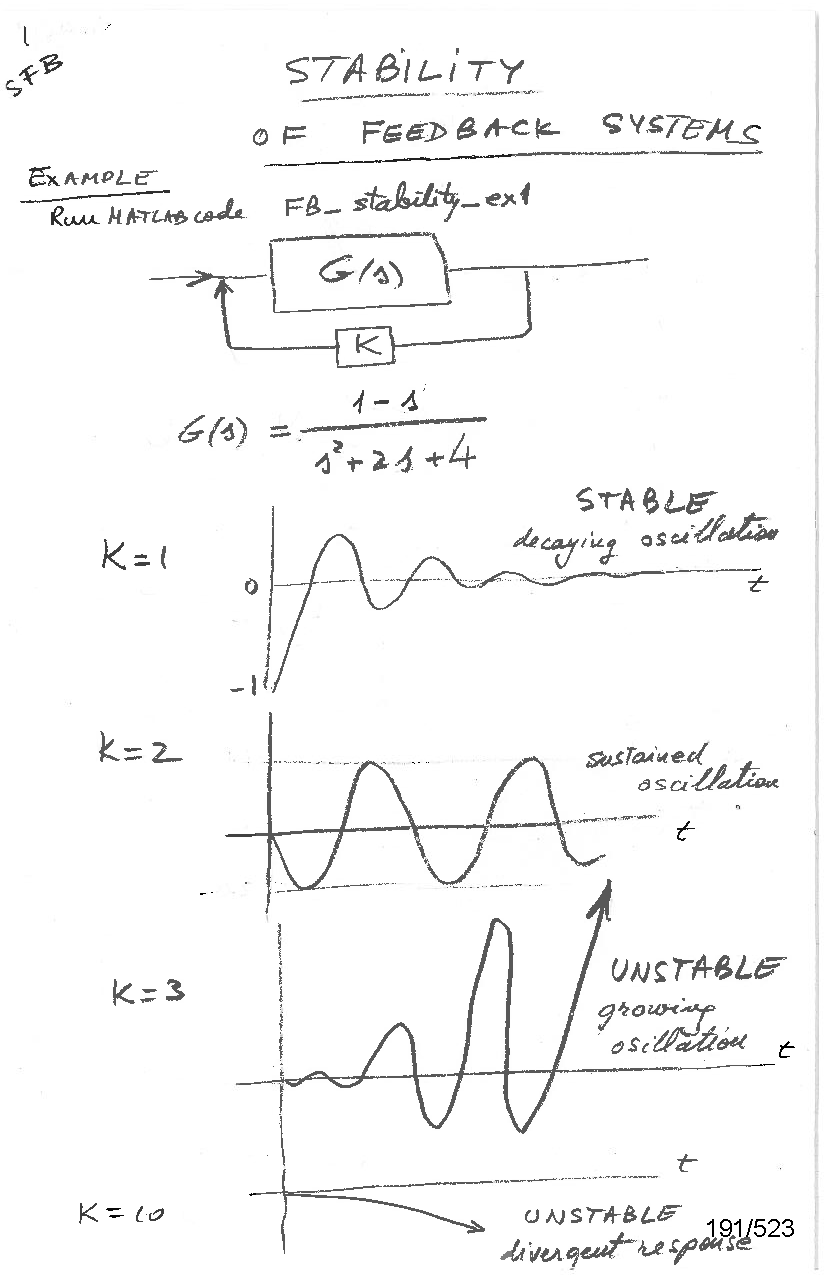
\includepdf[pages=-,pagecommand={},width=0.9\textwidth]{PDF_notes/Stability_of_feedback_control.pdf}

\subsection{Stability Criteria}
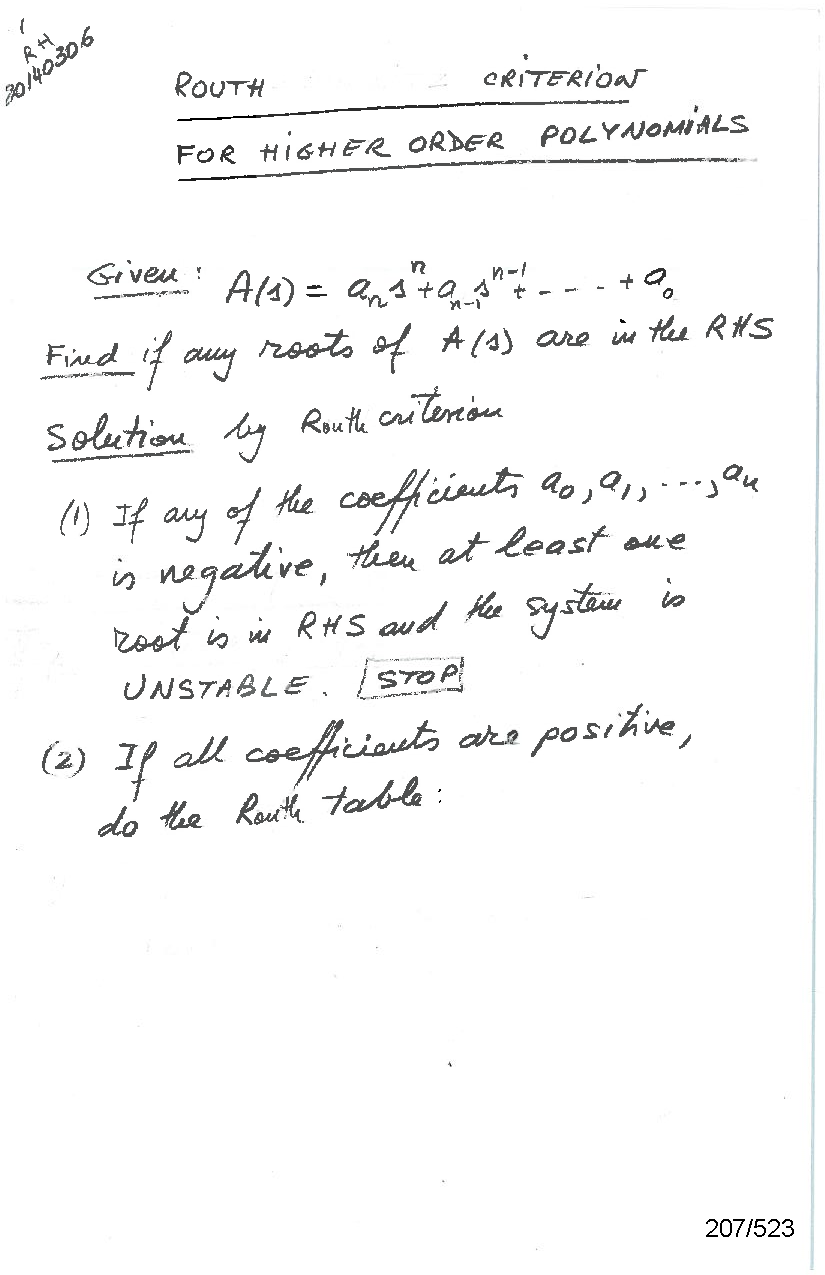
\includepdf[pages=-,pagecommand={},width=0.9\textwidth]{PDF_notes/Stability_Criteria.pdf}

\subsection{Feedback Controllers}
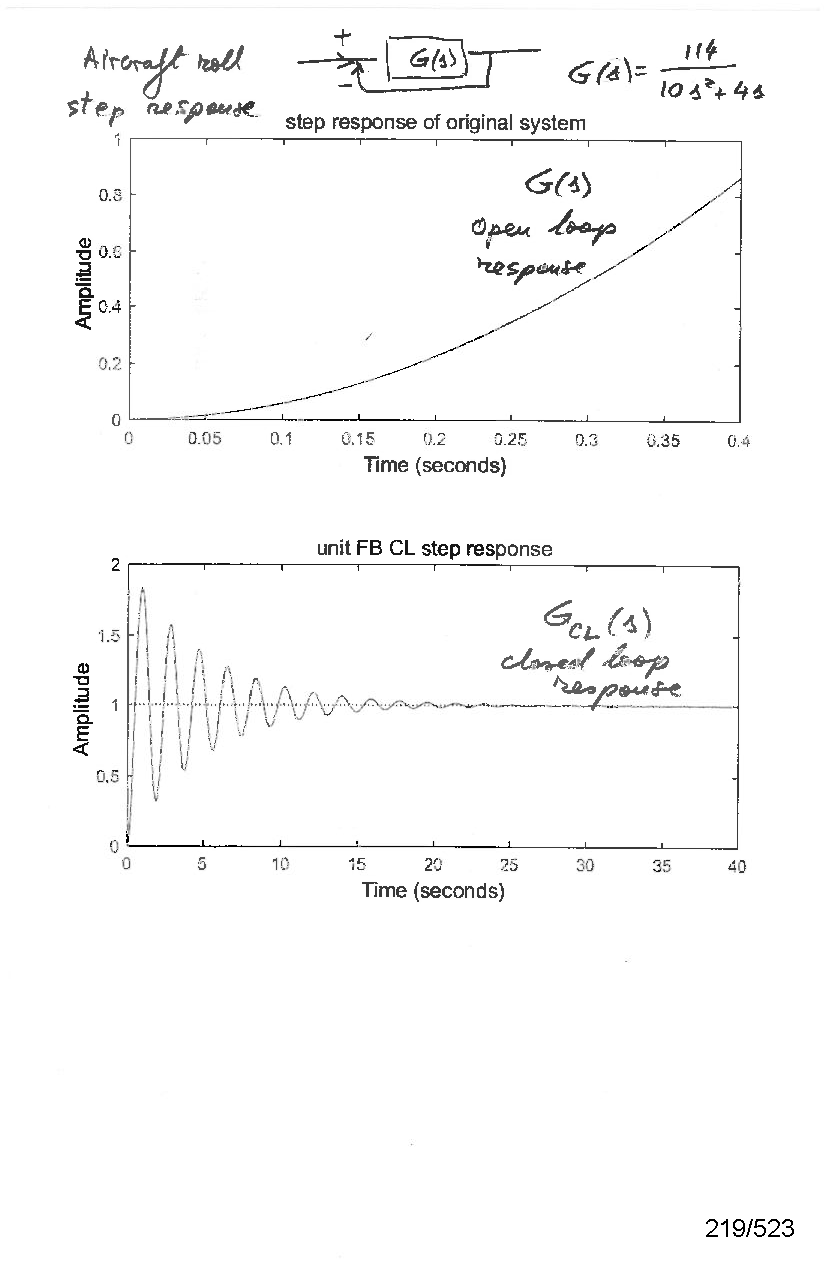
\includepdf[pages=-,pagecommand={},width=0.9\textwidth]{PDF_notes/Feedback_Controllers.pdf}

\subsection{SIMULINK Aircraft Roll Motion}
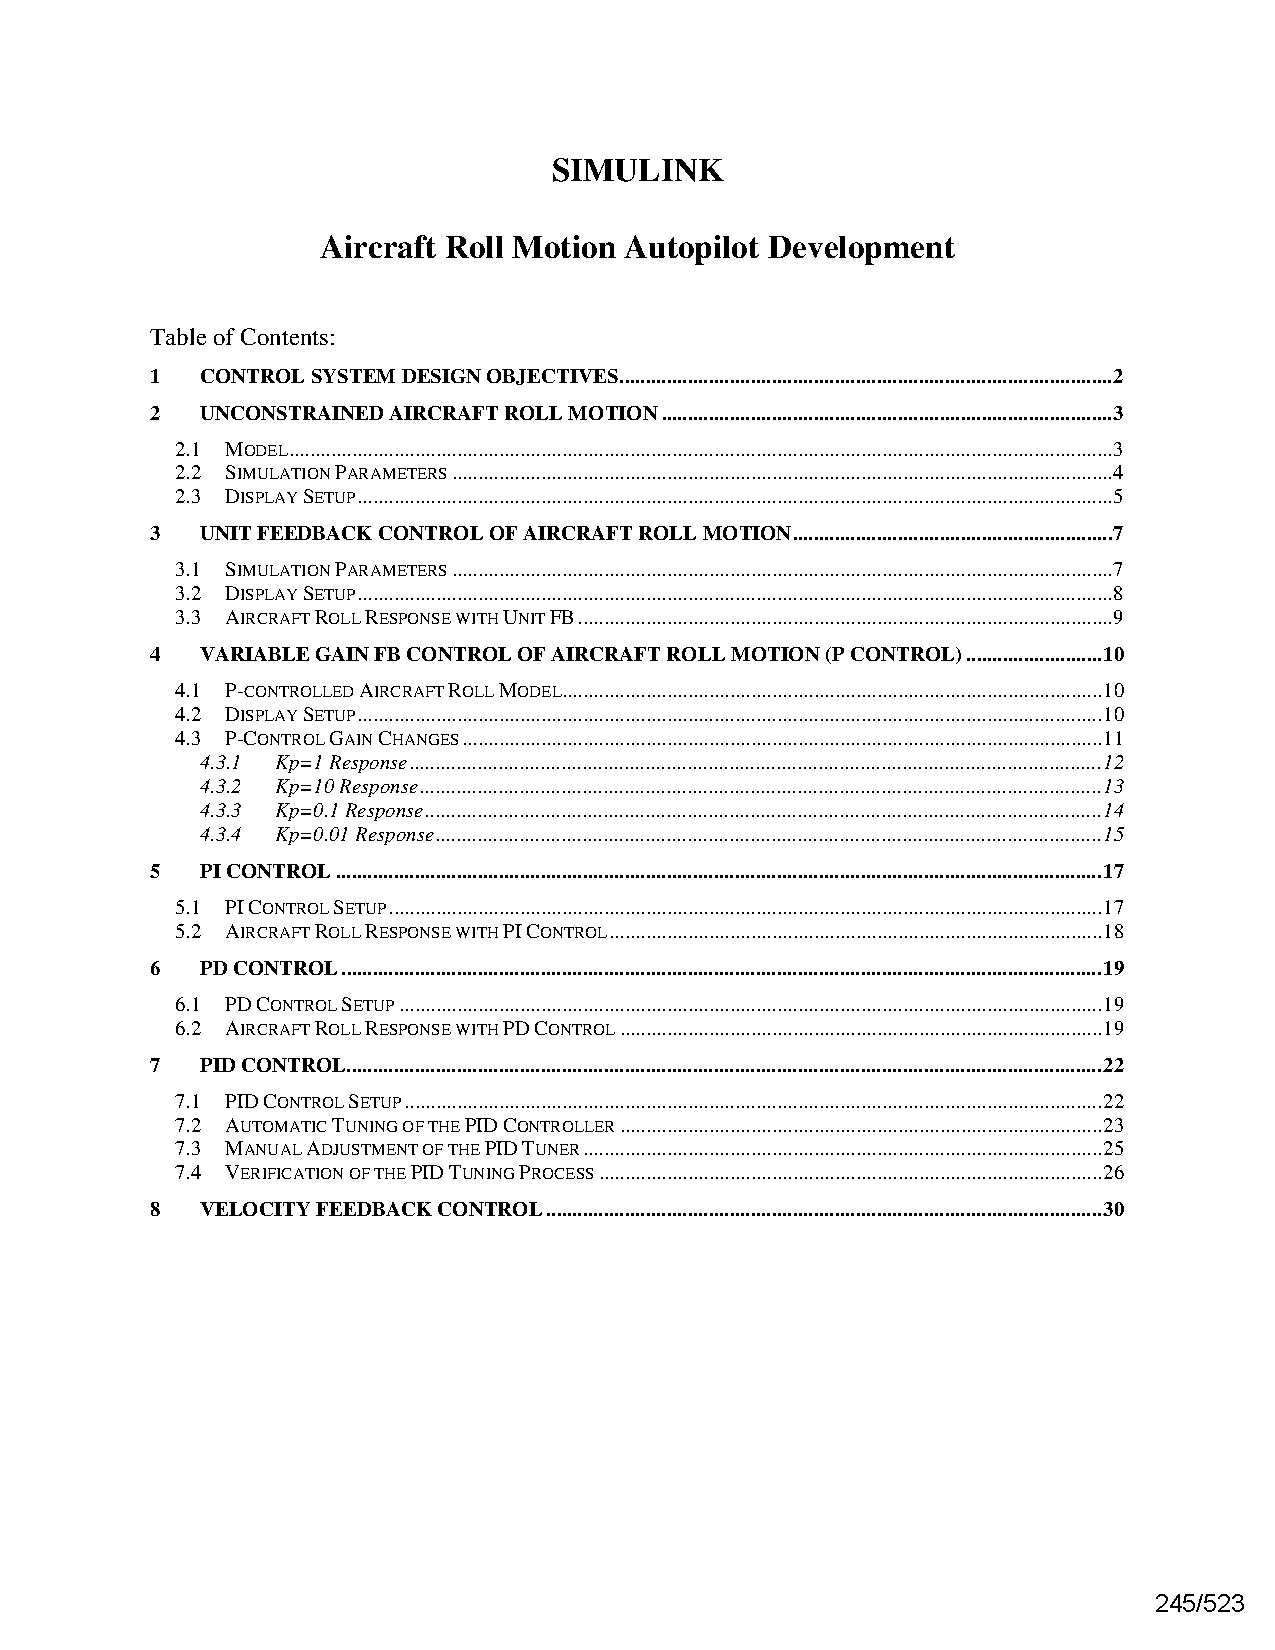
\includepdf[pages=-,pagecommand={},width=0.9\textwidth]{PDF_notes/SIMULINK_Aircraft_Roll_Motion.pdf}

\subsection{Feedback Controllers (continued)}
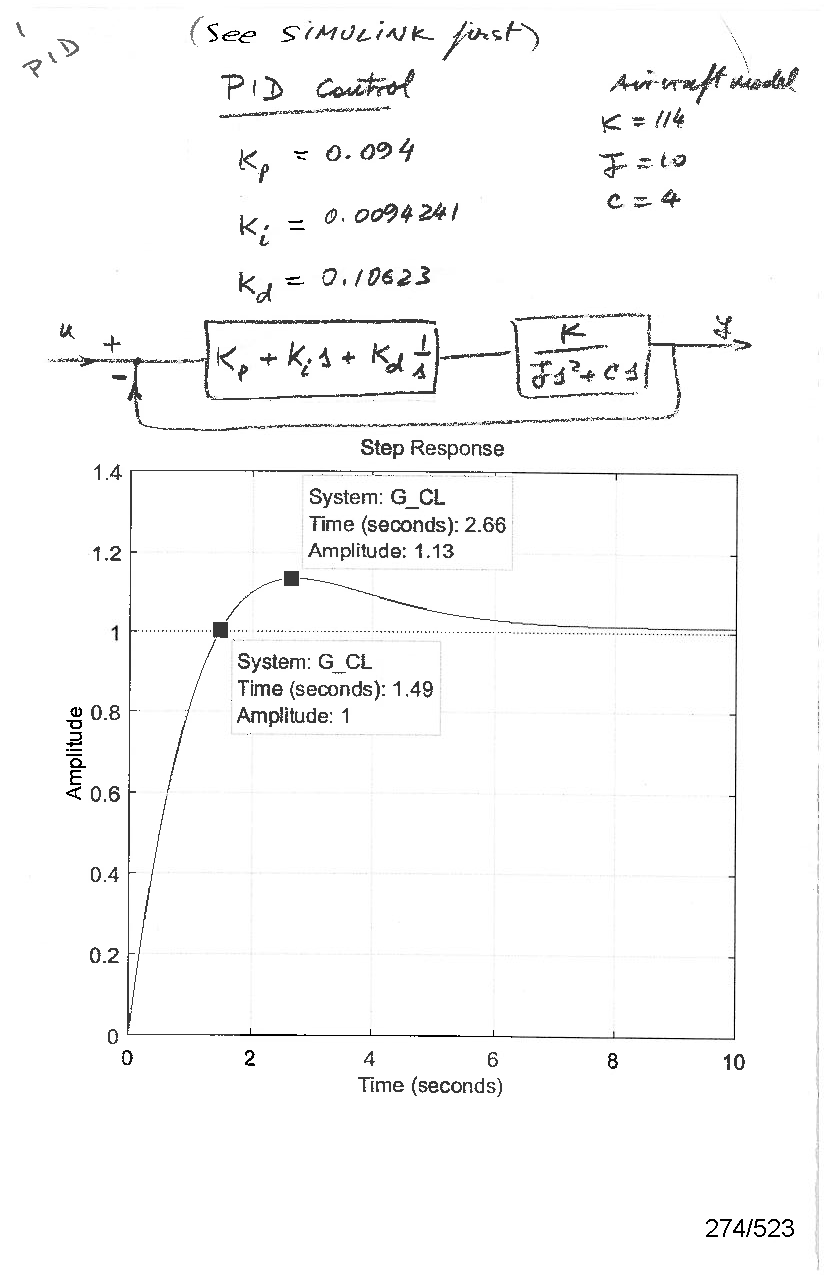
\includepdf[pages=-,pagecommand={},width=0.9\textwidth]{PDF_notes/Feedback_Controllers_continued.pdf}

\subsection{SIMULINK Aircraft Roll Motion (continued)}
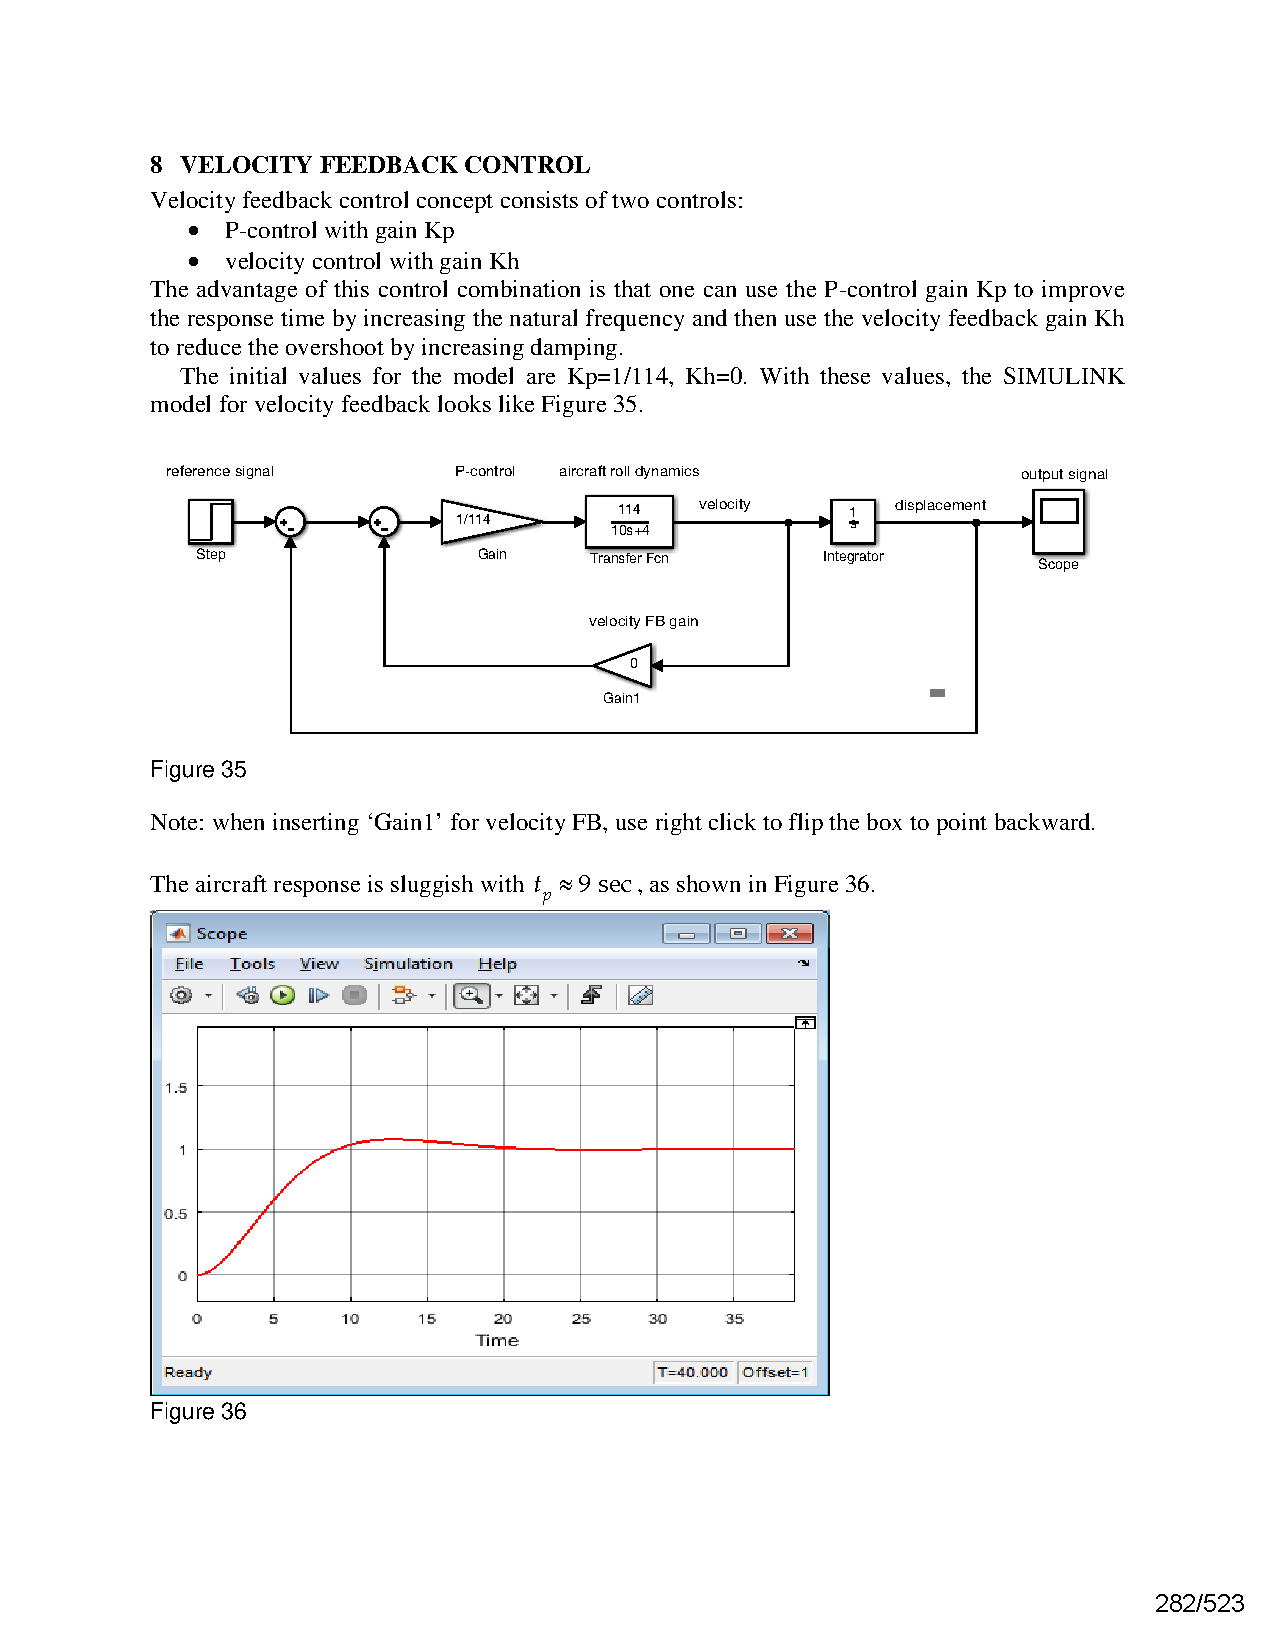
\includepdf[pages=-,pagecommand={},width=0.9\textwidth]{PDF_notes/SIMULINK_Aircraft_Roll_Motion_continued.pdf}

\subsection{Instability Suppression with velocity feedback}
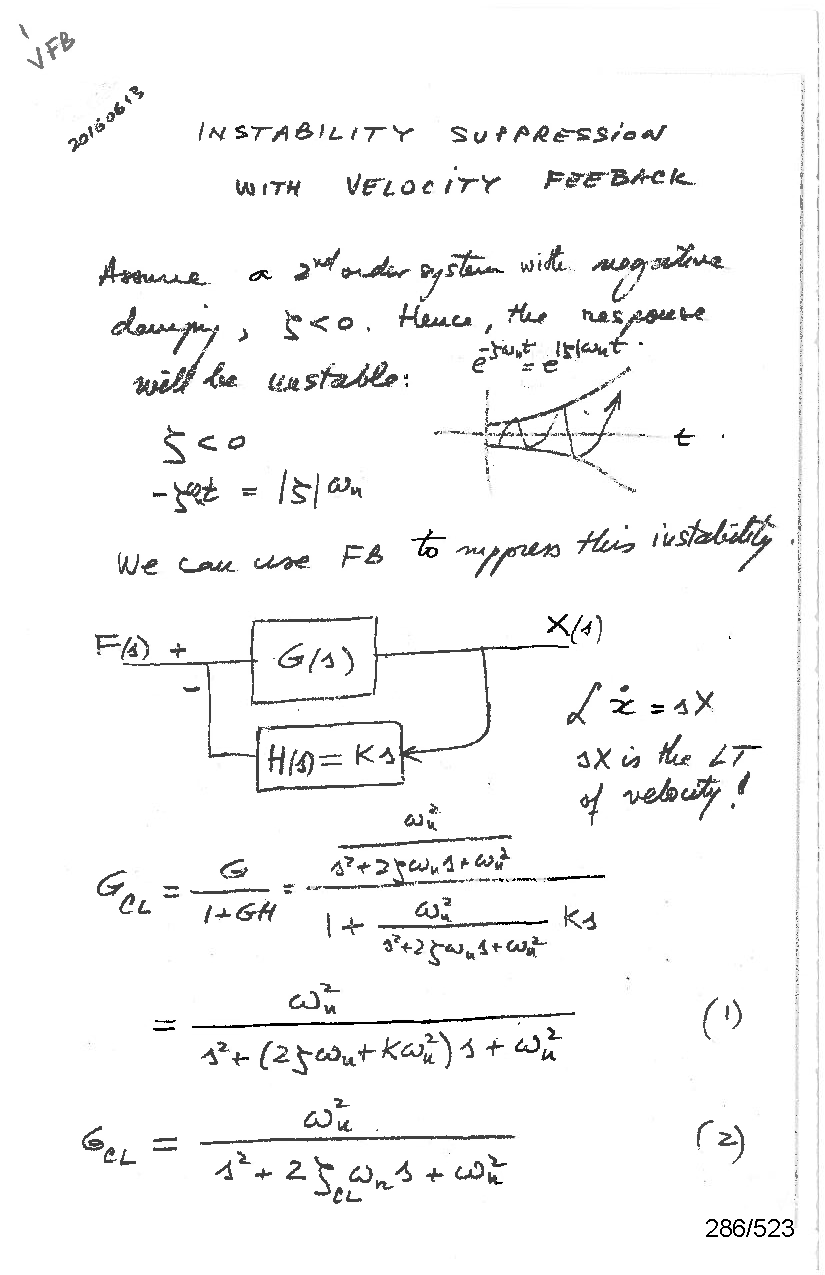
\includepdf[pages=-,pagecommand={},width=0.9\textwidth]{PDF_notes/Instability_Suppression.pdf}



	\pagebreak
	\renewcommand{\thepage}{}
	\renewcommand\refname{References Cited}
	\pagestyle{plain}
	\bibliographystyle{Downey_NSF}
	\bibliography{Chapter_1_Basic_Concepts}


















\end{document}

